\documentclass[10pt]{article}
\usepackage[margin=0.78in]{geometry}
\usepackage[T1]{fontenc}
\usepackage{lmodern}
\usepackage{amsmath,amssymb,booktabs,graphicx,xcolor}
\usepackage{microtype}
\usepackage{hyperref}
\usepackage{enumitem}
\usepackage{float}
\hypersetup{colorlinks=true,linkcolor=blue,urlcolor=blue}
\setlist{nosep,leftmargin=*}
\newcommand{\method}{\textsc{CoPH-Sense}}
\newcommand{\CVaR}{\operatorname{CVaR}}
\newcommand{\E}{\mathbb E}
\newcommand{\R}{\mathbb R}
\title{\vspace{-1.5em}\method: formulation and implementation progress\\
\large Research update relative to Prof. Bajaj's revised manuscript}
\author{Implementation progress report}
\date{17 September 2026}

\begin{document}
\maketitle
\vspace{-1.5em}
\begin{abstract}
The revised manuscript asks when a scout should acquire and share terrain
evidence so that a carrier can make a better \emph{physically executable}
decision under risk, resource, and communication constraints. We kept that
causal ordering and the port-Hamiltonian (pH)/MHRF execution backbone. We
first built exactly checkable finite tasks to validate set-valued sensing,
post-observation sharing, persistent memory, and communication deadlines;
then embodied those mechanisms in VMAS and integrated a fixed pH executor.
The main remaining gap is a valid, frozen procedural benchmark in which
physically acquiring complementary measurements is worthwhile often enough
to train and test the full learner. E2-Natural is frozen and legitimately
skip-heavy; the initial separate E2-Complementarity prototype has failed its
physical admission rule. No held-out off-road or full E2 learning advantage is
claimed here.
\end{abstract}

\section{Starting point and research question}
Prof. Bajaj's updated Overleaf manuscript frames a \emph{decentralized,
risk-sensitive, pH-executed information decision}: a scout can learn about a
future route before the carrier, but a measurement has value only if it can be
obtained, communicated, and used before the carrier loses the ability to
change maneuver. Sensing, detours, waiting, packet attempts, and both robots'
motion must be charged. The information policy is the new learning target;
the pH/MHRF controller is the inherited structured physical backbone. Our
implementation ladder tests the causal information mechanism before
claiming benefits in continuous unknown-terrain transport. This follows the
manuscript's architecture rather than replacing it with a classification-only
problem.\footnote{Source: revised
\texttt{Distributed-Co-PH-Riskv2/CoPH\_Sense\_ICLR2027\_Overleaf/}, especially
\texttt{core.tex} and \texttt{learning\_algorithm.tex}.}

\section{Notation, objective, and causal algorithm}
For agent $i\in\{s,c\}$ (scout, carrier), $x^i_t$ is its physical state and
$h^i_t$ its \emph{local} history of measurements, actions, and packets actually
delivered by time $t$. The latent map is
$M=(O,g,\mu)$: public static occupancy $O$, hidden surface condition $g$, and
hidden traction $\mu$. Let $b^i_t=P(M,x_t\mid h^i_t)$ denote the ideal local
belief (approximated in code), $D$ a feasible set of sensing actions, $Y_D$
their realized readings, and $E$ a subset of \emph{owned} evidence sent over
the declared packet channel. The carrier chooses a route/maneuver $\omega$;
the pH/MHRF layer produces an admissible force and executed control.

The manuscript's full target is a decentralized, finite-horizon objective
\begin{equation}
\min_{\pi\in\Pi_{\rm dec}}\sup_{P\in\mathfrak P}
\left\{\E_P[C_0(\pi)]+\lambda_R\CVaR^P_\alpha(C_R(\pi))\right\},
\quad
\CVaR_\alpha(Z)=\inf_\eta\left\{\eta+\frac{\E(Z-\eta)_+}{1-\alpha}\right\},
\label{eq:full}
\end{equation}
subject to failure, sensing, radio, and actuator/safety constraints. $C_0$
includes both agents' elapsed time/motion, sensing and communication charges,
and failure penalties. $C_R$ is cumulative material exposure. The current
E2 nominal decision score sets $\alpha=.95$ and $\lambda_R=1$ after fixed
normalization:
\begin{equation}
S(\mathcal I,D)=\E[C_0\mid\mathcal I,D]+\CVaR_{.95}(C_R\mid\mathcal I,D),\qquad
C_R=\frac{\Delta t}{T_{\max}}\sum_{k<T}\sum_{i\in\{s,c\}}r_{\rm true}(x^i_k),
\label{eq:e2score}
\end{equation}
where $r_{\rm true}=\mathrm{clip}(0.4g+0.4t+0.2gt,0,1)$ and
$t=\mathrm{clip}((0.55-\mu)/0.40,0,1)$. A finite teacher rollout uses the
same hidden world and random streams across actions, but the actor sees only
its own $h^i_t$. The full ambiguity-set supremum and mission-level safety
certificate in Eq.~\eqref{eq:full} are \emph{not} established by the current
VMAS experiments.

At a pre-acquisition information state $\mathcal I$, our restricted teacher
evaluates complete sensing sets under a specified continuation:
\begin{equation}
Q_{\rm sense}^{\pi}(\mathcal I,D)
=\E\!\left[C_{\rm travel+dwell+sensor}+C_{\rm packet}
 +C_{\rm remaining}^{\pi}\mid\mathcal I,\operatorname{do}(D)\right],\quad
D^*=\arg\min_{D\in\mathcal D(\mathcal I)}Q_{\rm sense}^{\pi}(\mathcal I,D).
\label{eq:qsense}
\end{equation}
After readings exist, $Q_{\rm share}(\mathcal I^y,E)$ compares sending them
with holding them under actual delay, range, and delivery. A positive
interaction
$Q_G+Q_T-Q_{GT}-Q_{\varnothing}>0$ means the pair saves more team cost than
the sum of its singleton improvements; it is \emph{not} guaranteed by merely
having two sensors. Acquisition regret always uses the same feasible menu and
continuation. Exact evaluation of a fixed policy is not exact optimization
over all decentralized policies.

\noindent\fbox{\begin{minipage}{0.965\linewidth}
\textbf{Algorithmic sequence (current implementation and intended extension).}
\begin{enumerate}[label=\arabic*.]
\item \textbf{Observe:} update each local belief/memory from its own sensors and
delivered packets with age and provenance; keep hidden truth evaluator-only.
\item \textbf{Acquire (A3/A5):} enumerate feasible $\varnothing$, singleton and
pair candidates; a variable-set critic predicts downstream mission cost and
risk-return quantiles. Charge travel, dwell, sensing, and lost actionability.
\item \textbf{Share (A4):} after the reading is realized, compare SEND/HOLD for
owned evidence. Requests do not reveal values; recipients update only on
packet delivery. Persistent memory changes later candidate values.
\item \textbf{Act:} use the post-delivery risk belief to choose a maneuver and
propose MHRF/pH motion. The full manuscript then applies its risk gate, energy
tank, and safety filter; the present VMAS bridge uses a fixed structured
executor, not the complete learned/certified controller.
\item \textbf{Train and check:} collect paired counterfactual returns on
training worlds, fit A3/A5 and A4, refresh labels on histories visited by the
learned stack, then evaluate complete decentralized rollouts. Freeze
calibration and held-out manifests before confirmatory E2 claims.
\end{enumerate}
\end{minipage}}

The physical backbone follows the manuscript's
$\dot z=[J(z)-R(z)]\nabla H(z)+Gu$ and its MHRF-style proposal
\begin{equation}
u_i^{\rm des}=u_i^0+\mathcal A_i\!\left[-g_i\lambda_i
\nabla_{q_i}\bar r_i(q_i;\hat b_i)+f_i^{\rm coord}\right].
\label{eq:ph}
\end{equation}
The proposed tank debits active-port power and storage jumps when the belief
or controller changes. Our current result verifies integration with a fixed
pH-style executor; it does not verify the entire tank/shield theorem in E2.

\section{Why the finite checkpoints came first}
The finite environments retain the manuscript's causal order while allowing
exact comparison of sensing and sharing branches. They expose failures that
a large navigation return could hide: leaked private evidence, a request
revealing a reading, a message arriving after a maneuver deadline, an
insufficient memory representation, or an optimistic A3 label that assumes
oracle A4 sharing. The moving VMAS bridge then tests whether those decisions
still matter when sensing and communication consume physical time. This is a
verification ladder toward the intended pH unknown-terrain application, not
a substitute for it.

\begin{table}[t]
\centering\small
\caption{Measured milestones. Numbers from different tasks have different
cost units and must not be compared across rows.}
\label{tab:milestones}
\begin{tabular}{p{0.13\linewidth}p{0.43\linewidth}p{0.35\linewidth}}
\toprule
Stage & Measured result & Scope / reading \\
\midrule
A0--A2 & Native pH-MARL VMAS checkpoint: final assignment distance 0.103 vs
0.900 random (10 matched seeds). Finite oracle: 4 worlds, 16 sensing subsets,
625 sharing policies; best cost 2.6874 vs 3.0000 no sensing. & Upstream native
checkpoint reproduced; finite oracle is an exactly enumerated diagnostic. \\
A3 & Pairwise set critic: acquisition regret $0.00423\pm0.00150$ over three
seeds (additive $0.01455\pm0.00485$). & Held-out finite teacher states;
not E2 navigation improvement. \\
A4 & Revised pairwise sharing critic: regret $0.01590$; critical-message
recall $99.33\%$, held-out warning recall $100\%$. & Post-reading finite
SEND/HOLD; repaired state sufficiency and warning coverage. \\
A5 & Learned memory-aware policy cost 5.2551, equal to restricted oracle;
independent 5.6600, shared-reset 5.7006; nested regret 0. & Exact finite
two-region task. Correct message changes the carrier's next measurement
from R1 to R2. \\
A6/A6.5 & Finite timing gate: $97.36\%$ decision agreement, regret 0.00182
vs 0.05885 always-inspect. Physical actionability gate: regret 0.0030 vs
0.0216 prior analytic VoI on a fresh 25-case set. & Deadline and moving
single-fork sanity checks; the actionability correction is analytic, not a
claimed learned contribution. \\
\bottomrule
\end{tabular}
\end{table}

\begin{figure}[H]
\centering
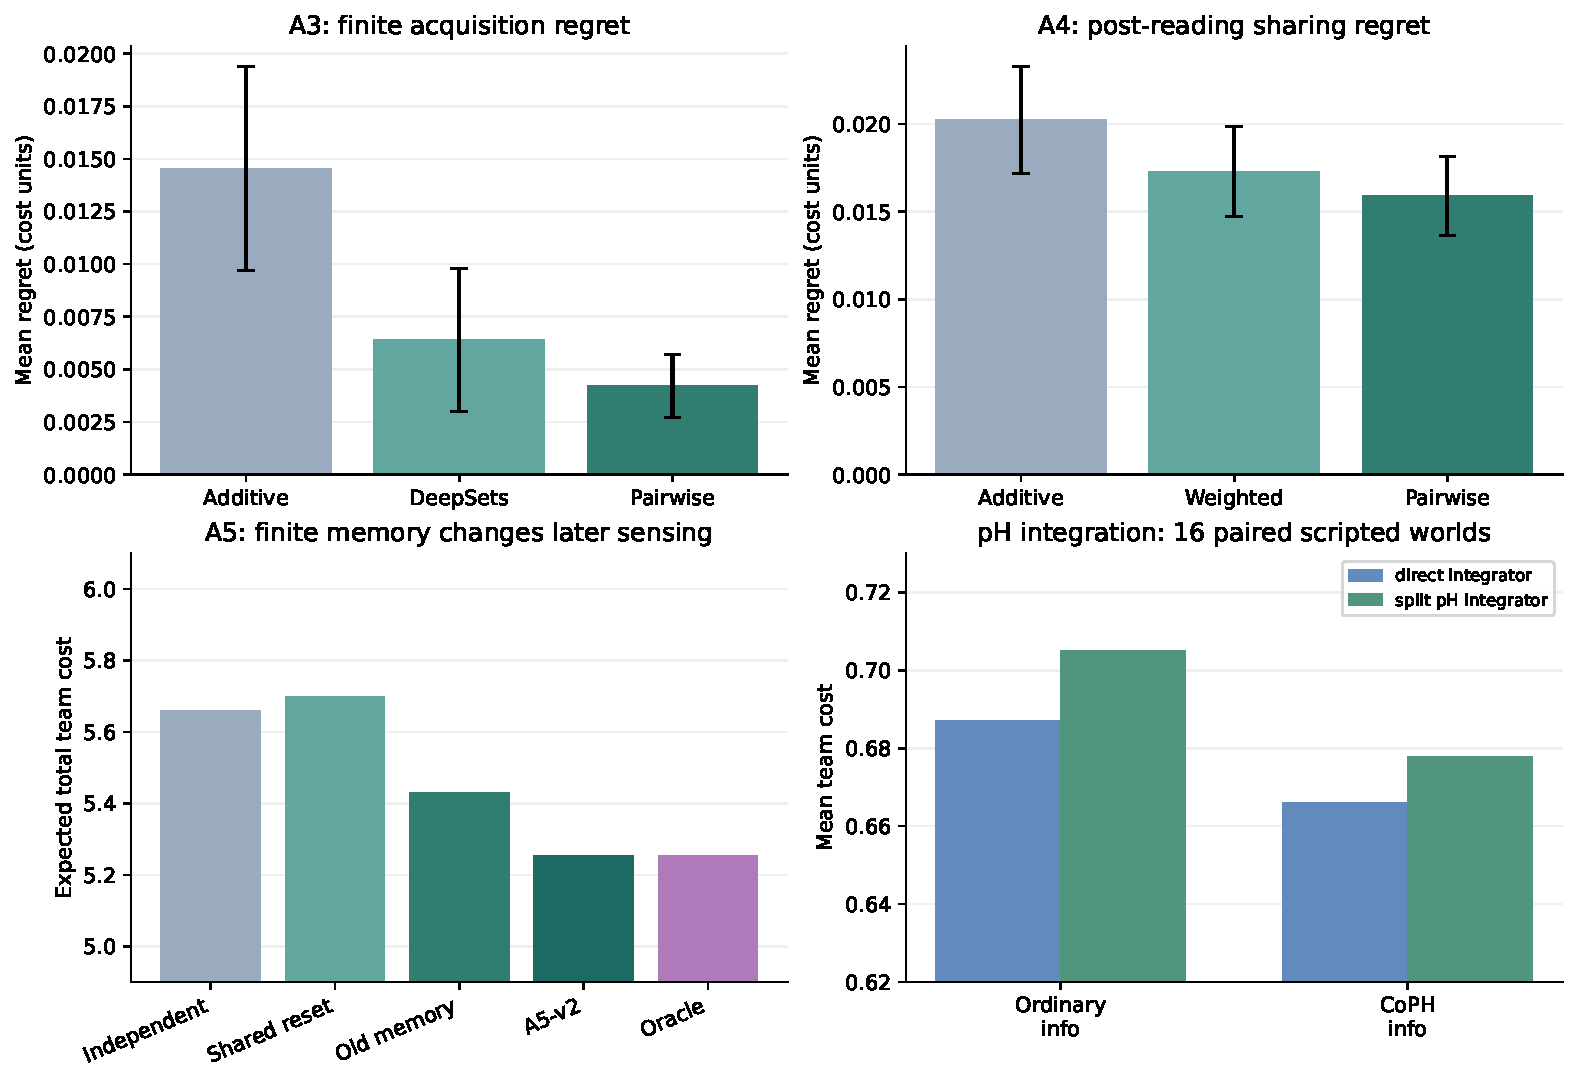
\includegraphics[width=.78\linewidth]{figures/progress_results.pdf}
\caption{Finite diagnostics and scripted pH integration, recreated from
saved result JSON. A3/A4 error bars are sample standard deviations across
three seeds; A5 is the exact finite expected cost; the factorial averages
16 paired worlds. The four panels have distinct scales and objectives.
The final panel compares two integrators of the \emph{same} continuous-time
pH vector field, not pH versus a structurally different non-pH controller.}
\label{fig:progress}
\end{figure}

\section{Embodied bridge and pH execution}
In the frozen two-fork scripted VMAS layout, the physical oracle chooses
Region~1 without scout memory ($Q=3.470$) and Region~2 after valid R1
evidence ($Q=2.634$). The unchanged frozen A5 critic makes both choices,
giving zero regret within this restricted menu. The matched safe-world
physical cost decreases by 0.2866. An archived canonical rollout records
actual scout G1/T1 acquisitions, two delivered packets, and carrier G2/T2
acquisitions; its completed team cost is 2.1163 versus 3.0894 for a
shared-reset replay that repeats R1. These are particular scripted-VMAS
branches, not generalization estimates.

The pH integration experiment holds the scripted worlds and information
interface fixed while varying ordinary versus CoPH information and direct
versus split numerical execution. Mean costs over 16 enumerated worlds are
\begin{center}\small
\begin{tabular}{lcc}\toprule
& Ordinary information & CoPH information \\\midrule
Direct integrator & 0.6871 & 0.6661 \\
Split pH integrator & 0.7051 & 0.6779 \\\bottomrule
\end{tabular}
\end{center}
The information effect is $-0.0209$ under direct execution and $-0.0272$
under split execution, with 16/16 successes in every cell. Sensing cost
(0.08) and communication cost (0.0488) are identical across cells, so this
experiment shows altered downstream physical behavior, not reduced sensing
or bytes. Since the two integrators share the same pH vector field, the
split-minus-direct difference is a \emph{numerical integration ablation};
it does not establish structural pH superiority.

\section{Procedural unknown terrain: layouts, data, and current evidence}
We then built a 12\,m $\times$ 12\,m VMAS scout--carrier world with public
static topology, hidden surface and traction, passive noisy appearance,
physical surface scans/contact traction probes, delayed charged packets,
deterministic replay, and a complete resource ledger. The pH executor is
kept fixed while the information policy is developed. The currently verified
Natural manifests contain 500 train, 100 validation, 100 calibration, 200
in-distribution test, and 200 OOD parent groups; the test splits are not
used for the engineering results here. RELLIS and TartanDrive remain planned
data-derived evaluation sources, not completed E2 experiments.

\begin{figure}[H]
\centering
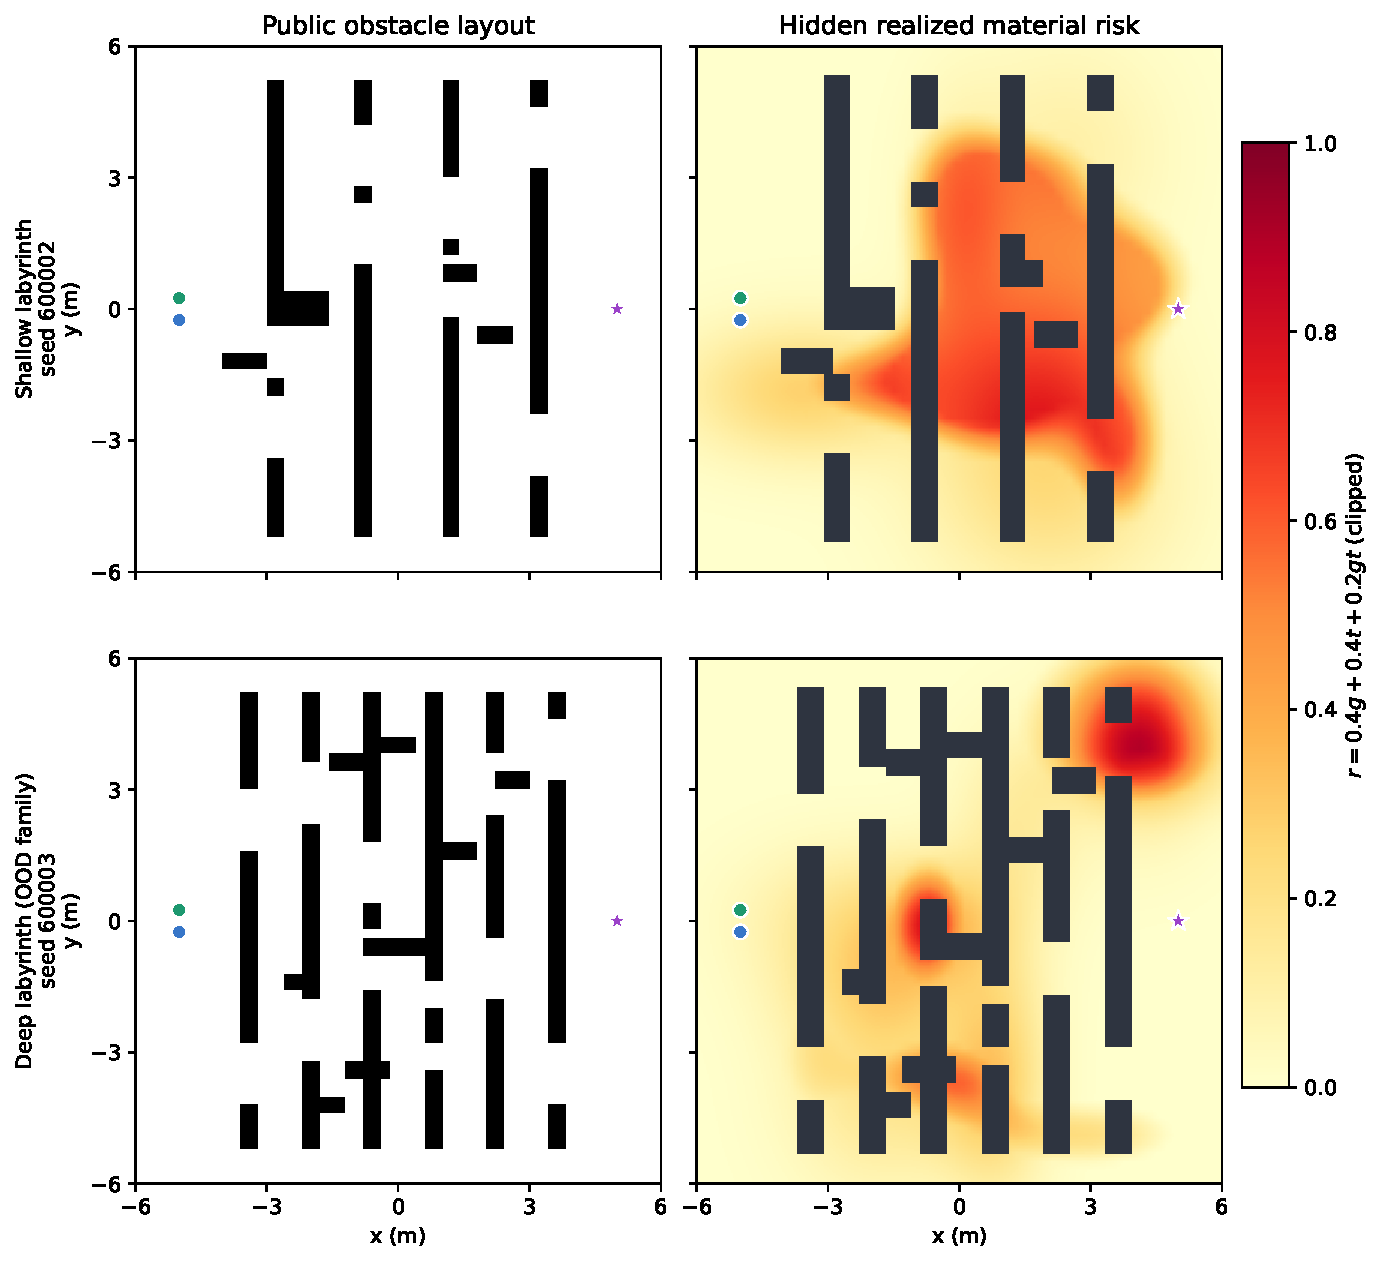
\includegraphics[width=.68\linewidth]{figures/maze_layouts_risk.pdf}
\caption{Current procedural shallow and deep labyrinth examples (seeds
600002/600003). Occupancy is public; colored material risk is hidden from
actors and plotted from evaluator truth only. Green/blue dots are scout and
carrier starts; purple stars are goals. Deep labyrinth is an OOD topology
family. The colorbar uses the current joint surface--traction risk formula.}
\label{fig:mazes}
\end{figure}

\begin{figure}[H]
\centering

\includegraphics[width=.80\linewidth]{figures/maze_information_flow_preview.png}
\caption{Qualitative information-flow replay in a labyrinth (parent seed
600042). Left is hidden true risk; middle and right are the separate local
maps of scout and carrier. Scripted physical acquisition and two delivered
packets make the carrier map update; with the same acquisitions, the paired
send continuation costs 1.9321 versus 2.4563 when evidence is withheld.
This illustrates the implemented causal path, \emph{not} that buying the pair
is optimal or that a learned E2 policy produced the trajectory.}
\label{fig:maze-flow}
\end{figure}

\section{Current blocker and next gate}
The predeclared fresh E2-Natural resource audit covered all 40 scheduled
states on 20 parent maps. Physical sensing beat skip by more than 0.01 in
only 2/39 evaluated decisions (5.13\%), below the 15\% nondegeneracy gate;
no pair was optimal. This is a valid result about the natural distribution:
many measurements cost more in travel, dwell, and delay than the future
decision benefit. We froze Natural instead of lowering prices or changing
risk to force positive labels. Its purpose is now to test sensible restraint,
success, cost, risk/CVaR, and resource use.

The separate controlled E2-Complementarity generator is still
\emph{provisional}. Admission uses an evaluator-only belief-expected physical
oracle across indistinguishable latent worlds, requires every branch to
succeed, both pair readings to be captured and delivered before region entry,
and a pair advantage greater than 0.02 over skip and either singleton.
It never screens on a CoPH checkpoint. The tested development parent failed:
\begin{center}\small
\begin{tabular}{lrrrrl}\toprule
Charged continuation & Skip & G & T & G+T & Outcome \\\midrule
Carrier moves & 1.2814 & 1.3534 & 1.3511 & 1.4543 & Pair loses; packets late \\
Carrier waits & 1.2814 & 1.4159 & 1.4408 & 4.2692 & One pair branch fails \\
\bottomrule
\end{tabular}
\end{center}
In the high-surface/high-traction-risk state, the waiting pair branch costs
12.6835 and does not deliver both readings. These maps are therefore
\emph{not} pair-positive training examples. Disposable teacher forcing does
execute an A4 SEND/HOLD comparison and a matched A5 retained/withheld state,
but its tested safe-world A4 label favors HOLD (1.0439 versus 1.1064 SEND).
Natural on-policy rollouts mostly skip, creating the expected coverage
chain: skip $\Rightarrow$ no reading $\Rightarrow$ no A4 state $\Rightarrow$
no delivered evidence $\Rightarrow$ no meaningful A5 state.

\textbf{Next gate.} Specify and freeze a separate physically feasible
Complementarity source pool, reporting its acceptance rate before fitting.
Then teacher-force \emph{training-only} acquisition to create real
post-reading A4 states and paired post-delivery A5 states; fit the shared
A3/A5 set critic and A4 critic on Natural-plus-challenge training states;
refresh on histories generated by the learned stack. Held-out regret for
A3/A4/A5 and a complete causal rollout must precede the matched rivals and
multi-seed campaign. The pH executor remains fixed through this information
learning step; optional pH proposal fine-tuning comes afterward. There is
currently no completed held-out E2-CoPH result.

\vspace{.3em}\noindent\textbf{Reproducibility.} This document, its figure
generator, and source JSON references are in
\path{reports/prof_progress_2026-09-17/}. The figures are regenerated
from saved finite/VMAS results and current terrain generator outputs.

\end{document}
